% Options for packages loaded elsewhere
\PassOptionsToPackage{unicode}{hyperref}
\PassOptionsToPackage{hyphens}{url}
\PassOptionsToPackage{dvipsnames,svgnames,x11names}{xcolor}
%
\documentclass[
  letterpaper,
  DIV=11,
  numbers=noendperiod]{scrartcl}

\usepackage{amsmath,amssymb}
\usepackage{iftex}
\ifPDFTeX
  \usepackage[T1]{fontenc}
  \usepackage[utf8]{inputenc}
  \usepackage{textcomp} % provide euro and other symbols
\else % if luatex or xetex
  \usepackage{unicode-math}
  \defaultfontfeatures{Scale=MatchLowercase}
  \defaultfontfeatures[\rmfamily]{Ligatures=TeX,Scale=1}
\fi
\usepackage{lmodern}
\ifPDFTeX\else  
    % xetex/luatex font selection
\fi
% Use upquote if available, for straight quotes in verbatim environments
\IfFileExists{upquote.sty}{\usepackage{upquote}}{}
\IfFileExists{microtype.sty}{% use microtype if available
  \usepackage[]{microtype}
  \UseMicrotypeSet[protrusion]{basicmath} % disable protrusion for tt fonts
}{}
\makeatletter
\@ifundefined{KOMAClassName}{% if non-KOMA class
  \IfFileExists{parskip.sty}{%
    \usepackage{parskip}
  }{% else
    \setlength{\parindent}{0pt}
    \setlength{\parskip}{6pt plus 2pt minus 1pt}}
}{% if KOMA class
  \KOMAoptions{parskip=half}}
\makeatother
\usepackage{xcolor}
\setlength{\emergencystretch}{3em} % prevent overfull lines
\setcounter{secnumdepth}{-\maxdimen} % remove section numbering
% Make \paragraph and \subparagraph free-standing
\makeatletter
\ifx\paragraph\undefined\else
  \let\oldparagraph\paragraph
  \renewcommand{\paragraph}{
    \@ifstar
      \xxxParagraphStar
      \xxxParagraphNoStar
  }
  \newcommand{\xxxParagraphStar}[1]{\oldparagraph*{#1}\mbox{}}
  \newcommand{\xxxParagraphNoStar}[1]{\oldparagraph{#1}\mbox{}}
\fi
\ifx\subparagraph\undefined\else
  \let\oldsubparagraph\subparagraph
  \renewcommand{\subparagraph}{
    \@ifstar
      \xxxSubParagraphStar
      \xxxSubParagraphNoStar
  }
  \newcommand{\xxxSubParagraphStar}[1]{\oldsubparagraph*{#1}\mbox{}}
  \newcommand{\xxxSubParagraphNoStar}[1]{\oldsubparagraph{#1}\mbox{}}
\fi
\makeatother

\usepackage{color}
\usepackage{fancyvrb}
\newcommand{\VerbBar}{|}
\newcommand{\VERB}{\Verb[commandchars=\\\{\}]}
\DefineVerbatimEnvironment{Highlighting}{Verbatim}{commandchars=\\\{\}}
% Add ',fontsize=\small' for more characters per line
\usepackage{framed}
\definecolor{shadecolor}{RGB}{241,243,245}
\newenvironment{Shaded}{\begin{snugshade}}{\end{snugshade}}
\newcommand{\AlertTok}[1]{\textcolor[rgb]{0.68,0.00,0.00}{#1}}
\newcommand{\AnnotationTok}[1]{\textcolor[rgb]{0.37,0.37,0.37}{#1}}
\newcommand{\AttributeTok}[1]{\textcolor[rgb]{0.40,0.45,0.13}{#1}}
\newcommand{\BaseNTok}[1]{\textcolor[rgb]{0.68,0.00,0.00}{#1}}
\newcommand{\BuiltInTok}[1]{\textcolor[rgb]{0.00,0.23,0.31}{#1}}
\newcommand{\CharTok}[1]{\textcolor[rgb]{0.13,0.47,0.30}{#1}}
\newcommand{\CommentTok}[1]{\textcolor[rgb]{0.37,0.37,0.37}{#1}}
\newcommand{\CommentVarTok}[1]{\textcolor[rgb]{0.37,0.37,0.37}{\textit{#1}}}
\newcommand{\ConstantTok}[1]{\textcolor[rgb]{0.56,0.35,0.01}{#1}}
\newcommand{\ControlFlowTok}[1]{\textcolor[rgb]{0.00,0.23,0.31}{\textbf{#1}}}
\newcommand{\DataTypeTok}[1]{\textcolor[rgb]{0.68,0.00,0.00}{#1}}
\newcommand{\DecValTok}[1]{\textcolor[rgb]{0.68,0.00,0.00}{#1}}
\newcommand{\DocumentationTok}[1]{\textcolor[rgb]{0.37,0.37,0.37}{\textit{#1}}}
\newcommand{\ErrorTok}[1]{\textcolor[rgb]{0.68,0.00,0.00}{#1}}
\newcommand{\ExtensionTok}[1]{\textcolor[rgb]{0.00,0.23,0.31}{#1}}
\newcommand{\FloatTok}[1]{\textcolor[rgb]{0.68,0.00,0.00}{#1}}
\newcommand{\FunctionTok}[1]{\textcolor[rgb]{0.28,0.35,0.67}{#1}}
\newcommand{\ImportTok}[1]{\textcolor[rgb]{0.00,0.46,0.62}{#1}}
\newcommand{\InformationTok}[1]{\textcolor[rgb]{0.37,0.37,0.37}{#1}}
\newcommand{\KeywordTok}[1]{\textcolor[rgb]{0.00,0.23,0.31}{\textbf{#1}}}
\newcommand{\NormalTok}[1]{\textcolor[rgb]{0.00,0.23,0.31}{#1}}
\newcommand{\OperatorTok}[1]{\textcolor[rgb]{0.37,0.37,0.37}{#1}}
\newcommand{\OtherTok}[1]{\textcolor[rgb]{0.00,0.23,0.31}{#1}}
\newcommand{\PreprocessorTok}[1]{\textcolor[rgb]{0.68,0.00,0.00}{#1}}
\newcommand{\RegionMarkerTok}[1]{\textcolor[rgb]{0.00,0.23,0.31}{#1}}
\newcommand{\SpecialCharTok}[1]{\textcolor[rgb]{0.37,0.37,0.37}{#1}}
\newcommand{\SpecialStringTok}[1]{\textcolor[rgb]{0.13,0.47,0.30}{#1}}
\newcommand{\StringTok}[1]{\textcolor[rgb]{0.13,0.47,0.30}{#1}}
\newcommand{\VariableTok}[1]{\textcolor[rgb]{0.07,0.07,0.07}{#1}}
\newcommand{\VerbatimStringTok}[1]{\textcolor[rgb]{0.13,0.47,0.30}{#1}}
\newcommand{\WarningTok}[1]{\textcolor[rgb]{0.37,0.37,0.37}{\textit{#1}}}

\providecommand{\tightlist}{%
  \setlength{\itemsep}{0pt}\setlength{\parskip}{0pt}}\usepackage{longtable,booktabs,array}
\usepackage{calc} % for calculating minipage widths
% Correct order of tables after \paragraph or \subparagraph
\usepackage{etoolbox}
\makeatletter
\patchcmd\longtable{\par}{\if@noskipsec\mbox{}\fi\par}{}{}
\makeatother
% Allow footnotes in longtable head/foot
\IfFileExists{footnotehyper.sty}{\usepackage{footnotehyper}}{\usepackage{footnote}}
\makesavenoteenv{longtable}
\usepackage{graphicx}
\makeatletter
\newsavebox\pandoc@box
\newcommand*\pandocbounded[1]{% scales image to fit in text height/width
  \sbox\pandoc@box{#1}%
  \Gscale@div\@tempa{\textheight}{\dimexpr\ht\pandoc@box+\dp\pandoc@box\relax}%
  \Gscale@div\@tempb{\linewidth}{\wd\pandoc@box}%
  \ifdim\@tempb\p@<\@tempa\p@\let\@tempa\@tempb\fi% select the smaller of both
  \ifdim\@tempa\p@<\p@\scalebox{\@tempa}{\usebox\pandoc@box}%
  \else\usebox{\pandoc@box}%
  \fi%
}
% Set default figure placement to htbp
\def\fps@figure{htbp}
\makeatother
% definitions for citeproc citations
\NewDocumentCommand\citeproctext{}{}
\NewDocumentCommand\citeproc{mm}{%
  \begingroup\def\citeproctext{#2}\cite{#1}\endgroup}
\makeatletter
 % allow citations to break across lines
 \let\@cite@ofmt\@firstofone
 % avoid brackets around text for \cite:
 \def\@biblabel#1{}
 \def\@cite#1#2{{#1\if@tempswa , #2\fi}}
\makeatother
\newlength{\cslhangindent}
\setlength{\cslhangindent}{1.5em}
\newlength{\csllabelwidth}
\setlength{\csllabelwidth}{3em}
\newenvironment{CSLReferences}[2] % #1 hanging-indent, #2 entry-spacing
 {\begin{list}{}{%
  \setlength{\itemindent}{0pt}
  \setlength{\leftmargin}{0pt}
  \setlength{\parsep}{0pt}
  % turn on hanging indent if param 1 is 1
  \ifodd #1
   \setlength{\leftmargin}{\cslhangindent}
   \setlength{\itemindent}{-1\cslhangindent}
  \fi
  % set entry spacing
  \setlength{\itemsep}{#2\baselineskip}}}
 {\end{list}}
\usepackage{calc}
\newcommand{\CSLBlock}[1]{\hfill\break\parbox[t]{\linewidth}{\strut\ignorespaces#1\strut}}
\newcommand{\CSLLeftMargin}[1]{\parbox[t]{\csllabelwidth}{\strut#1\strut}}
\newcommand{\CSLRightInline}[1]{\parbox[t]{\linewidth - \csllabelwidth}{\strut#1\strut}}
\newcommand{\CSLIndent}[1]{\hspace{\cslhangindent}#1}

\KOMAoption{captions}{tableheading}
\makeatletter
\@ifpackageloaded{caption}{}{\usepackage{caption}}
\AtBeginDocument{%
\ifdefined\contentsname
  \renewcommand*\contentsname{Table of contents}
\else
  \newcommand\contentsname{Table of contents}
\fi
\ifdefined\listfigurename
  \renewcommand*\listfigurename{List of Figures}
\else
  \newcommand\listfigurename{List of Figures}
\fi
\ifdefined\listtablename
  \renewcommand*\listtablename{List of Tables}
\else
  \newcommand\listtablename{List of Tables}
\fi
\ifdefined\figurename
  \renewcommand*\figurename{Figure}
\else
  \newcommand\figurename{Figure}
\fi
\ifdefined\tablename
  \renewcommand*\tablename{Table}
\else
  \newcommand\tablename{Table}
\fi
}
\@ifpackageloaded{float}{}{\usepackage{float}}
\floatstyle{ruled}
\@ifundefined{c@chapter}{\newfloat{codelisting}{h}{lop}}{\newfloat{codelisting}{h}{lop}[chapter]}
\floatname{codelisting}{Listing}
\newcommand*\listoflistings{\listof{codelisting}{List of Listings}}
\makeatother
\makeatletter
\makeatother
\makeatletter
\@ifpackageloaded{caption}{}{\usepackage{caption}}
\@ifpackageloaded{subcaption}{}{\usepackage{subcaption}}
\makeatother

\usepackage{bookmark}

\IfFileExists{xurl.sty}{\usepackage{xurl}}{} % add URL line breaks if available
\urlstyle{same} % disable monospaced font for URLs
\hypersetup{
  pdftitle={Association Between individual Health Management, Income, and Insurance Coverage in Preventive Healthcare Among U.S. Adults},
  pdfauthor={Sandesh Manjunath Raykar; Daniel Lee},
  pdfkeywords={health effort, income, checkup},
  colorlinks=true,
  linkcolor={blue},
  filecolor={Maroon},
  citecolor={Blue},
  urlcolor={Blue},
  pdfcreator={LaTeX via pandoc}}


\title{Association Between individual Health Management, Income, and
Insurance Coverage in Preventive Healthcare Among U.S. Adults}
\author{Sandesh Manjunath Raykar \and Daniel Lee}
\date{}

\begin{document}
\maketitle
\begin{abstract}
This study examines two interrelated questions using data from the
2016--2017 American Health Values Survey (AHVS), a nationally
representative dataset of U.S. adults collected by NORC at the
University of Chicago. The first question investigates whether
individuals who report putting greater effort into managing their
personal health---through behaviors such as regular exercise, healthy
eating, stress reduction, and routine medical engagement---are less
likely to have been diagnosed by a doctor with high blood pressure. The
second question explores how annual household income and insurance
coverage are associated with the time since an individual's last routine
medical checkup, reflecting differences in access to preventive
healthcare services across socioeconomic groups.

To address these questions, the analysis employs logistic regression to
estimate the odds of receiving a high blood pressure diagnosis as a
function of self-reported health management, and ordinal regression to
model the relationship between household income, insurance status, and
the recency of preventive medical visits. Results indicate that
individuals who engage more actively in managing their health report
significantly lower odds of having been diagnosed with high blood
pressure, even after accounting for demographic factors. Similarly,
adults with higher household incomes and health insurance coverage are
substantially more likely to have had a recent routine checkup compared
to lower-income or uninsured respondents.

Overall, these findings highlight important behavioral and socioeconomic
disparities in preventive health and chronic disease outcomes. The
results suggest that both individual lifestyle management and structural
access to care play critical roles in promoting better health and
reducing inequalities within the U.S. healthcare system.
\end{abstract}


\subsection{Introduction and Background}\label{sec-intro}

Preventive healthcare plays a critical role in early disease detection
and reducing long-term health costs. Regular checkups, screenings, and
healthy lifestyle behaviors help identify potential health risks before
they become serious, ultimately improving quality of life and reducing
the financial burden on individuals and the healthcare system. Despite
these benefits, engagement in preventive health practices varies widely
among Americans, reflecting differences in awareness, motivation, and
access to care.

To better understand patterns in Americans health, this study takes two
complementary perspectives. The first focuses on individual effort to
maintain or improve health, capturing personal behaviors such as
exercise, healthy eating, and proactive health management. The second
examines access to routine medical checkups influenced by income level,
representing the structural and socioeconomic conditions that shape
preventive healthcare utilization. Together, these perspectives provide
a more holistic understanding of how both personal and contextual
factors contribute to preventive health outcomes in the United States.

Preventive healthcare plays a critical role in early disease detection
and reducing long-term health costs . Regular checkups, screenings, and
healthy lifestyle behaviors help identify potential health risks before
they become serious, ultimately improving quality of life and reducing
the financial burden on individuals and the healthcare system. Despite
these benefits, engagement in preventive health practices varies widely
among Americans, reflecting differences in awareness, motivation, and
access to care. Research consistently shows that Wilcox et al.
(\citeproc{ref-wilcox2000}{2000}) individuals who engage in consistent
health-promoting behaviors, such as maintaining a balanced diet,
exercising regularly, practicing stress management through meditation,
and adhering to preventive medical routines, experience better long-term
health outcomes. These include lower risks of chronic diseases such as
hypertension, diabetes, and heart disease, as well as improved mental
well-being and functional health throughout adulthood.

Previous research Rentfrow et al. (\citeproc{ref-rentfrow2013}{2013})
shows that family income strongly influences access to medical care and
preventive services. Adults with lower income levels face greater
barriers to care, often forgoing medical visits or prescriptions due to
cost, while even brief insurance disruptions reduce preventive services
such as routine checkups. Building on this evidence, the present study
investigates how socioeconoㅁmic factors---particularly annual household
income---relate to both health effort and the time since one's last
routine checkup. By analyzing these relationships, this study seeks to
highlight socioeconomic disparities in preventive healthcare among U.S.
adults and contribute to a deeper understanding of the behavioral and
structural determinants of health.

\subsection{Study Design and Data collection}\label{sec-design}

This study employs a cross-sectional observational design using data
from the 2016--2017 American Health Values Survey, a nationally
representative dataset of U.S. adults. The analysis focuses on
respondents aged 18 and older who provided complete information on key
variables, including self-reported effort in maintaining the health,
blood pressure diagnosis, annual household income, and time since last
routine medical checkup. Data were collected through structured survey
questionnaires administered online and by phone, ensuring coverage
across diverse demographic and socioeconomic groups. This design allows
for examining associations between behavioral and socioeconomic factors
and health outcomes without manipulating variables or establishing
causality.

This study utilized a cross-sectional observational design drawing upon
data from the 2016--2017 American Health Values Survey (AHVS), conducted
by NORC at the University of Chicago with support from the Robert Wood
Johnson Foundation. The AHVS is a nationally representative survey
designed to assess the health beliefs, values, and behaviors of U.S.
adults across diverse demographic and regional contexts. The analysis in
this study was restricted to respondents aged 18 years and older who
provided complete responses to key variables, including self-reported
health effort, blood pressure diagnosis, annual household income, and
time since last routine medical checkup.

Data were collected using a multimode survey design, incorporating
online (CAWI), mail (self-administered paper questionnaires), and
telephone interviews (CATI). This mixed-method approach enhanced
accessibility for respondents with varying levels of internet access and
literacy, ensuring more comprehensive coverage across urban and rural
populations. The survey was available in both English and Spanish, and
participants received small prepaid and contingent incentives to improve
response rates

According to the AHVS and the related Sentinel Community Surveys
collected detailed information on participants' health values, personal
health priorities, self-efficacy, access to care, and social
determinants of health. The structured questionnaire captured both
quantitative and categorical data, allowing for the examination of
associations between behavioral, social, and economic factors and
various health outcomes without any manipulation of variables. Because
of its cross-sectional nature, this design allows for identifying
correlations and group differences but does not infer causality.

\subsection{Methods}\label{methods}

\paragraph{Data Preparation}\label{sec-dataprep-methods}

Data for this study were obtained from the 2016--2017 American Health
Values Survey. The dataset was first cleaned and filtered to include
only respondents aged 18 years and older to focus the analysis on
adults. Observations with missing or incomplete responses for key
analytical variables---specifically health effort, annual household
income, and time since last routine medical checkup---were excluded to
ensure data quality and consistency. This filtering process helped
minimize bias that could result from incomplete information.

Before computing summary measures, several data-cleaning procedures were
implemented. Responses coded as 77 (``Don't know'') or 99 (``No
answer'') were treated as invalid and replaced with missing values (NA)
across relevant variables, particularly the health activity items
(act1--act7) that contributed to the health effort measure. A new
variable, healtheffort, was then created as the mean of act1 through
act7 for each respondent, with missing values excluded from the
calculation. This variable reflects an individual's overall effort
toward maintaining or improving their health.

The income and checkup variables underwent the same cleaning and
recoding procedures. Responses coded as 77 (``Don't know'') and 99
(``Refused'') were treated as missing values (NA). The income variable
was categorized into eight ordered levels, ranging from less than
\$15,000 to \$150,000 or more, while the checkup variable was recoded
into five ordered groups, from within the past year to never. Data
integrity checks were then performed to ensure that all invalid codes
were removed and all transformations were accurately implemented. These
procedures produced a reliable dataset suitable for statistical analysis
and modeling.

\paragraph{Statistical Analysis}\label{sec-analysis-methods}

The statistical analysis for this study was guided by the analytical
framework used in the American Health Values Survey (AHVS) and the
Sentinel Community Health Values Surveys (SCHVS). The AHVS employed
k-means clustering, a widely used unsupervised classification technique,
to identify distinct groups of respondents based on their health values,
beliefs, and behaviors. This method partitions the dataset into k
mutually exclusive clusters by minimizing the within-cluster variance
while maximizing the differences between cluster centroids.

Following the AHVS methodology, several solutions ranging from four to
ten clusters were examined to determine the most meaningful group
segmentation. The final cluster solution was selected based on
statistical indicators such as the cubic clustering criterion and the
Pseudo F statistic, ensuring that the identified typology best captured
variation in respondents' health attitudes and behaviors. Demographic
and descriptive measures were then compared across clusters to confirm
the face validity of the typology, ensuring that the observed groupings
aligned with known differences in health, political, and socioeconomic
characteristics among U.S. adults.

For the present analysis using the cleaned AHVS dataset, descriptive
statistics were first computed to summarize respondent demographics and
key health indicators (e.g., health effort, income level, and time since
last routine checkup). Bivariate tests, including chi-square and
correlation analyses, were used to assess relationships between
categorical and continuous variables. Where applicable, multiple linear
and logistic regression models were applied to examine associations
between behavioral and socioeconomic predictors and health outcomes such
as blood pressure diagnosis, while controlling for demographic
covariates. All data cleaning, transformation, and analyses were
performed using R (version 4.3.2). The tidyverse, dplyr, and ggplot2
packages were utilized for data manipulation and visualization, while
stats functions supported regression modeling and significance testing.
Statistical significance was set at p \textless{} 0.05.

\subsection{Results}\label{sec-results}

\begin{figure}

\centering{

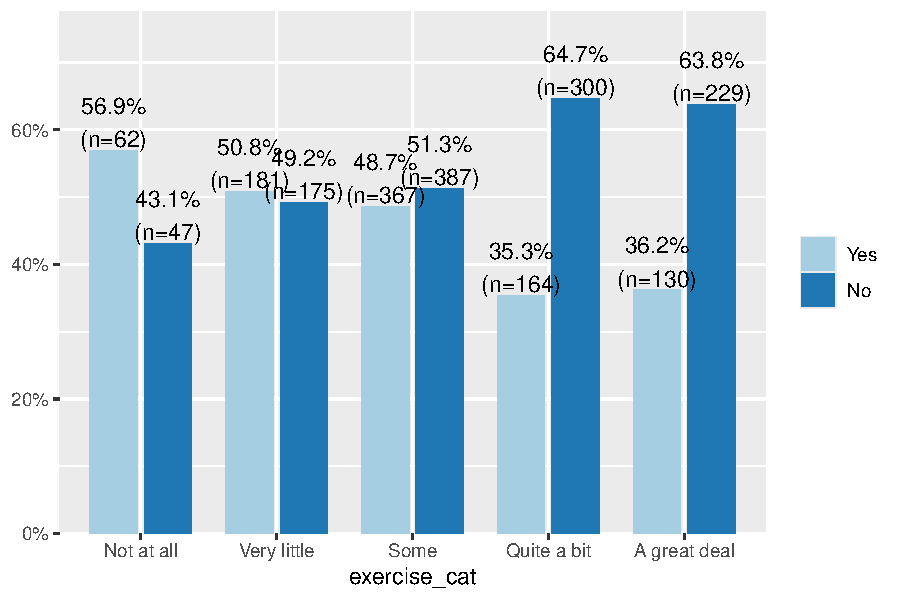
\includegraphics[width=0.7\linewidth,height=\textheight,keepaspectratio]{template_files/figure-pdf/fig-exercise-1.pdf}

}

\caption{\label{fig-exercise}Relationship between exercise effort and
high blood pressure diagnosis.}

\end{figure}%

The bar chart illustrates the relationship between self-reported
exercise effort and whether respondents reported a diagnosis of high
blood pressure. Each bar shows the percentage of respondents in each
exercise category (``Not at all'' to ``A great deal'') who reported
having or not having high blood pressure.

As the graph shows, individuals who reported doing more exercise were
less likely to have been diagnosed with high blood pressure. For
example, among those who reported exercising ``a great deal,'' only
36.2\% had high blood pressure, compared to 56.9\% among those who did
not exercise at all. This downward trend suggests that greater physical
activity is associated with a lower likelihood of high blood pressure,
supporting well-established evidence that regular exercise helps
regulate blood pressure and improve cardiovascular health.

\subsection{Discussion, Conclusion}\label{sec-discussino}

The results of this study reveal two key patterns linking behavioral and
socioeconomic factors to preventive health outcomes among U.S. adults.
First, individuals who reported putting greater effort into managing
their personal health---through activities such as regular exercise,
healthy eating, stress management, and proactive medical care---were
significantly less likely to report a diagnosis of high blood pressure.
This finding aligns with existing research demonstrating that consistent
engagement in healthy behaviors helps regulate blood pressure, improve
cardiovascular function, and reduce the risk of chronic disease. It
reinforces the importance of self-care practices as an essential
component of preventive healthcare, suggesting that promoting active
health management could lead to improved long-term health outcomes and
reduced healthcare costs.

Second, the analysis showed that household income and health insurance
coverage were strong predictors of preventive healthcare utilization.
Participants with higher income levels and stable insurance coverage
were more likely to have received a recent routine medical checkup
compared to those with lower income or no insurance. This pattern
supports prior evidence that financial resources and access to care
remain major determinants of preventive health engagement. The results
highlight ongoing socioeconomic disparities in the U.S. healthcare
system, where lower-income individuals may delay or forgo preventive
visits due to cost, lack of coverage, or competing life demands.

Despite these meaningful insights, several limitations should be noted.
The study's cross-sectional design prevents establishing causal
relationships between health effort, income, and health outcomes. The
use of self-reported data may also introduce recall or social
desirability bias, as individuals may overstate their healthy behaviors.
Additionally, unmeasured factors such as education, neighborhood
environment, or stress levels may influence both health behavior and
outcomes.

Future research should explore these relationships using longitudinal
data to better understand how personal health management and
socioeconomic conditions interact over time. Including more detailed
measures of lifestyle behaviors, health literacy, and psychological
well-being could further clarify the mechanisms linking preventive
efforts and health outcomes. Such work would strengthen the evidence
base for policies and interventions aimed at improving access to
preventive care and promoting equitable health behaviors across income
groups.

\subsection{Appendix}\label{appendix}

\begin{Shaded}
\begin{Highlighting}[]
\NormalTok{sjPlot}\SpecialCharTok{::}\FunctionTok{plot\_xtab}\NormalTok{(}\AttributeTok{grp=}\NormalTok{clean}\SpecialCharTok{$}\NormalTok{bp\_cat, }\AttributeTok{x=}\NormalTok{clean}\SpecialCharTok{$}\NormalTok{exercise\_cat, }
                  \AttributeTok{show.total =} \ConstantTok{FALSE}\NormalTok{, }\AttributeTok{margin=}\StringTok{"row"}\NormalTok{, }\AttributeTok{legend.title=}\StringTok{""}\NormalTok{) }
\end{Highlighting}
\end{Shaded}

\subsection*{References}\label{references}
\addcontentsline{toc}{subsection}{References}

\phantomsection\label{refs}
\begin{CSLReferences}{1}{0}
\bibitem[\citeproctext]{ref-rentfrow2013}
Rentfrow, P. J., S. D. Gosling, M. Jokela, D. J. Stillwell, M. Kosinski,
and J. Potter. 2013. {``Divided We Stand: Three Psychological Regions of
the United States and Their Correlates.''} \emph{Journal of Personality
and Social Psychology} 105 (6): 996--1012.

\bibitem[\citeproctext]{ref-wilcox2000}
Wilcox, S., C. Castro, A. C. King, R. Housemann, and R. C. Brownson.
2000. {``Determinants of Leisure-Time Physical Activity in Rural Vs.
Urban Older Women.''} \emph{Journal of Epidemiology \& Community Health}
54 (9): 667--72.

\end{CSLReferences}




\end{document}
